\begin{center}
    \Huge{\textbf{\underline{Chapter 1: Introduction}}}
\end{center}

\setcounter{section}{0}

\vspace{0.35cm}

\section{Steps Of An Attack}

\vspace{0.25cm}
\begin{center}
    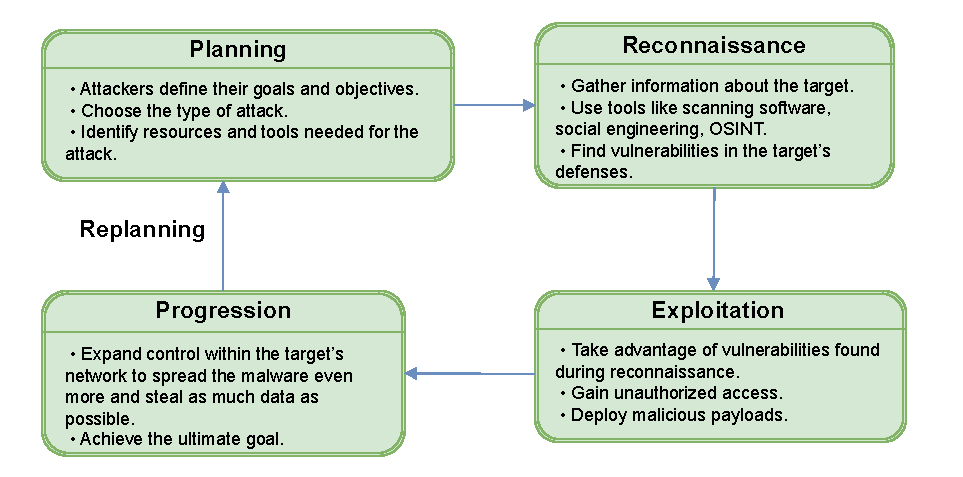
\includegraphics[width=0.9\textwidth]{Chapters/Diagram/Introduction/attack.drawio.pdf}
\end{center}

\vspace{0.35cm}
\section{Reasons for Poor Security}
\begin{prettyBox}{Reasons}{myblue}
\begin{itemize}
    \item \textbf{Insufficient Budget}: Approximately \(\frac{1}{4}\) of issues arise due to inadequate funding for cybersecurity initiatives and personnel.
    \item \textbf{Unqualified Personnel}: A lack of skilled and properly trained cybersecurity professionals.
    \item \textbf{Poor Administration}: Inefficient management and lack of synchronization in security policies and practices.
\end{itemize}
\end{prettyBox}

\vspace{0.35cm}

\section{Impacts of a Cyberattack}
\begin{prettyBox}{Impacts}{myblue}
\begin{itemize}
    \item \textbf{Data Breach}: Unauthorized access to sensitive client or organizational data. This may include\\ encrypting data for ransom (ransomware), sharing confidential information, or selling it on the dark web.  
    \item \textbf{Denial of Service (DoS)}: Disrupting or halting the services of an organization, making them inaccessible to users.   
    \item \textbf{Financial Loss}: Hacking into bank accounts, demanding ransom (ransomware attacks), or causing service interruptions that result in revenue loss.  
    \item \textbf{Damage to Reputation}: Eroding client trust or tarnishing someone's reputation by exposing compromised or sensitive data.  
    \item \textbf{Loss of Clients}: Organizations may lose clients due to the exposure of sensitive information, compromised systems, server outages, and interruptions in services.  
\end{itemize}
\end{prettyBox}

\newpage

\section{Information System}
\begin{prettyBox}{Definition}{myblue}
A set of active applications, services, and other components that allow for the management of informations.
Vulnerabilities can affect all components of the information system (IS).  
\end{prettyBox}

\section{Responses to Cyberattacks}
\begin{prettyBox}{Responses}{myblue}
\begin{itemize}
    \item \textbf{Reduce the Impact}: Taking measures to minimize the damage caused by the cyberattack, such as isolating affected systems, restoring backups, or limiting access.  
    \item \textbf{Accept the Risk}: The least effective response, where no action is taken to counter the attack. This could include surrendering to attackers’ demands, such as paying a ransom.  
    \item \textbf{Refuse or Resolve the Risk}: Actively countering the attack by refusing to comply with attackers and taking corrective actions to fix vulnerabilities or breaches.  
    \item \textbf{Transfer the Responsibility}: Shifting the burden of dealing with the cyberattack to a third party, such as an insurance provider or a managed cybersecurity service.  
\end{itemize}
\end{prettyBox}

\vspace{0.5cm}

\section{Steps For Protection (Deming's Wheel)}
\begin{prettyBox}{PDCA}{myblue}
    The PDCA (Plan-Do-Check-Act) cycle is a continuous improvement process widely used in
cybersecurity to ensure effective protection and adapt to evolving threats. Below are the four key steps:

    \begin{itemize}
        \item \textbf{\textcolor{green}{P}lan}: Identify goals, assess risks, and develop strategies to strengthen cybersecurity.
        \item \textbf{\textcolor{green}{D}o}: Implement the cybersecurity measures, like deploying firewalls and training staff.
        \item \textbf{\textcolor{green}{C}heck}: Monitor and evaluate the effectiveness of security measures through audits and testing.
        \item \textbf{\textcolor{green}{A}ct}: Address weaknesses and refine security measures to adapt to new threats.
    \end{itemize}
\end{prettyBox}

\begin{center}
    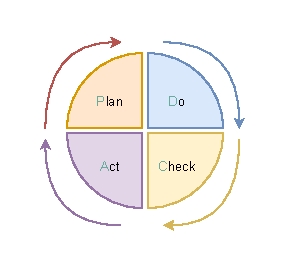
\includegraphics[width=0.5\textwidth]{Chapters/Diagram/Introduction/pdca.drawio.pdf}
\end{center}


